
%(BEGIN_QUESTION)
% Copyright 2011, Tony R. Kuphaldt, released under the Creative Commons Attribution License (v 1.0)
% This means you may do almost anything with this work of mine, so long as you give me proper credit

Undersøk tilstanden til dette væskeoppvarmingssystemet:

$$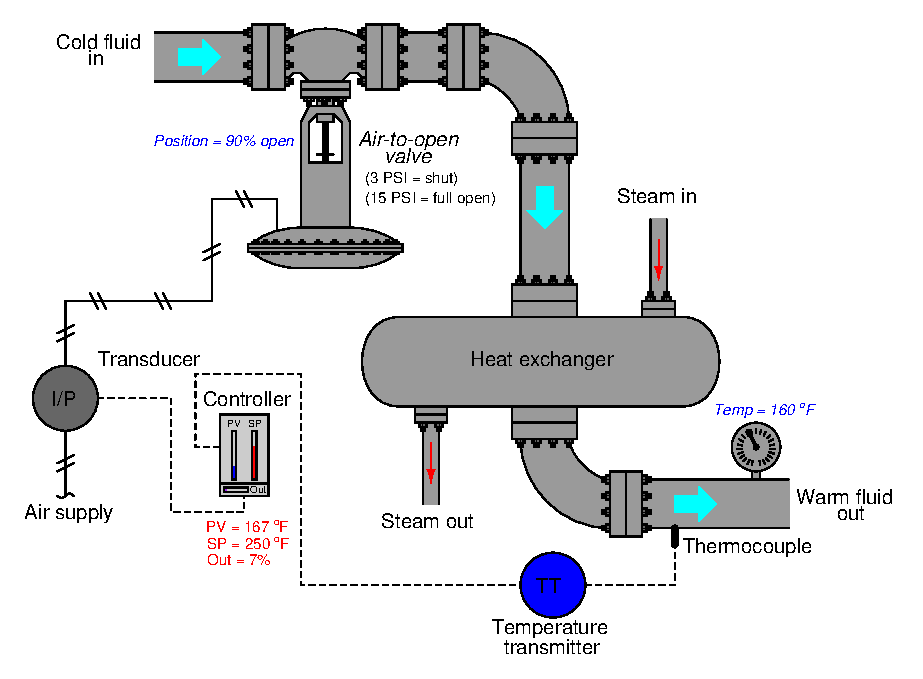
\includegraphics[width=15.5cm]{i00010x01.eps}$$

Temperaturen på væsken ut er godt under settpunktet, så vi vet at det er et problem et sted i systemet.

Bestem den diagnostiske verdien av hver av følgende tester.  Anta kun én feil i systemet, inkludert enhver enkelt komponent eller en enkelt ledning/kabel/slange som forbinder komponenter sammen.  Hvis en foreslått test kan gi ny informasjon som hjelper deg å identifisere plasseringen og/eller naturen til den ene feilen, merk "ja".  Hvis en foreslått test ikke vil avdekke noe relevant for å identifisere feilen (allerede forståelig ut fra målingene og symptomene gitt så langt), merk "nei".

% No blank lines allowed between lines of an \halign structure!
% I use comments (%) instead, so that TeX doesn't choke.

$$\vbox{\offinterlineskip
\halign{\strut
\vrule \quad\hfil # \ \hfil & 
\vrule \quad\hfil # \ \hfil & 
\vrule \quad\hfil # \ \hfil \vrule \cr
\noalign{\hrule}
%
% First row
{\bf Diagnostisk test} & {\bf Ja} & {\bf Nei} \cr
%
\noalign{\hrule}
%
% Another row
Mål millivolt-signal fra termoelementet &  &  \cr
%
\noalign{\hrule}
%
% Another row
Mål 4-20 mA-signal fra TT &  &  \cr
%
\noalign{\hrule}
%
% Another row
Mål 4-20 mA-signal fra regulatoren &  &  \cr
%
\noalign{\hrule}
%
% Another row
Mål instrumentluft-tilførselstrykk til I/P &  &  \cr
%
\noalign{\hrule}
%
% Another row
Mål 3-15 PSI-signal fra I/P &  &  \cr
%
\noalign{\hrule}
%
% Another row
Mål temperaturen på innkommende damp og sammenlign med normal &  &  \cr
%
\noalign{\hrule}
} % End of \halign 
}$$ % End of \vbox

Forklar også begrunnelsen for å anta kun {\it én} feil når du først diagnostiserer et systemproblem.  Hvorfor ikke holde muligheten åpen for {\it flere} feil når du vurderer mulige årsaker i starten?

\vfil

\underbar{file i00010}
\eject
%(END_QUESTION)





%(BEGIN_ANSWER)

Dette er et vurdert spørsmål -- ingen svar eller hint gis!

%(END_ANSWER)





%(BEGIN_NOTES)

Sammenligner vi regulatorens utgangssignal (7\%) med faktisk ventilposisjon (90\%), ser vi et stort avvik.  Derfor ligger problemet et sted i utgangshalvdelen av dette kontrollsystemet (mellom regulator og ventil, inkludert).  Det at feilen ligger i utgangshalvdelen gjør at vi kan se bort fra tester som kun gjelder inngangssiden (målesiden).

\vskip 10pt

Enten står ventilen fast åpen, eller noe er galt med regulatoren eller I/P som gir for høyt pneumatisk trykk til ventilen.  Enhver test som kan hjelpe oss å avgjøre om regulatoren gir feil milliamp-signal, eller om I/P gir feil PSI-signal, er en gyldig test.

% No blank lines allowed between lines of an \halign structure!
% I use comments (%) instead, so that TeX doesn't choke.

$$\vbox{\offinterlineskip
\halign{\strut
\vrule \quad\hfil # \ \hfil & 
\vrule \quad\hfil # \ \hfil & 
\vrule \quad\hfil # \ \hfil \vrule \cr
\noalign{\hrule}
%
% First row
{\bf Diagnostisk test} & {\bf Ja} & {\bf Nei} \cr
%
\noalign{\hrule}
%
% Another row
Mål millivolt-signal fra termoelementet &  & $\surd$ \cr
%
\noalign{\hrule}
%
% Another row
Mål 4-20 mA-signal fra TT &  & $\surd$ \cr
%
\noalign{\hrule}
%
% Another row
Mål 4-20 mA-signal fra regulatoren & $\surd$ &  \cr
%
\noalign{\hrule}
%
% Another row
Mål instrumentluft-tilførselstrykk til I/P & ? &  \cr
%
\noalign{\hrule}
%
% Another row
Mål 3-15 PSI-signal fra I/P & $\surd$ &  \cr
%
\noalign{\hrule}
%
% Another row
Mål temperaturen på innkommende damp og sammenlign med normal &  & $\surd$ \cr
%
\noalign{\hrule}
} % End of \halign 
}$$ % End of \vbox

Testen med å måle tilført lufttrykk er merket med "?" i stedet for kryss, fordi den er langt mindre sannsynlig å avsløre problemet.  For høyt tilførselstrykk {\it kan} skade I/P slik at den gir høyere utgangstrykk enn den skal, men uten å vite mer om I/P sin interne konstruksjon er det vanskelig å si om denne muligheten er sannsynlig nok til å være verdt seriøs vurdering.

\vskip 10pt

Sannsynligheten for flere uavhengige (tilfeldige) feil er mye lavere enn sannsynligheten for én enkelt feil, og derfor bør dette være den {\it første} antakelsen ved feilsøking.  Først når hypotesen om én feil er utprøvd, bør du vurdere flere feil.

%INDEX% Basics, control loop troubleshooting: isolating area of fault by correspondence

%(END_NOTES)
